\documentclass[a4paper,9pt]{extarticle}

%=========================================================
% PACKAGES
%=========================================================

\usepackage[
a4paper,
top=1.8cm,
bottom=1.5cm,
footskip=7mm,
left=1cm,
right=1cm,
headheight=14pt,
headsep=5mm
]{geometry}
\usepackage[T1]{fontenc}
\usepackage[utf8]{inputenc}
\usepackage[french]{babel}

\usepackage[sfdefault]{FiraSans}
\renewcommand{\familydefault}{\sfdefault}

\usepackage{multicol}
\setlength{\columnsep}{0.7cm}

\usepackage{amsmath,amssymb}

\usepackage{titlesec}
\usepackage{enumitem}

\usepackage{tcolorbox}
\tcbuselibrary{skins,breakable}

\usepackage{xcolor}

\usepackage{graphicx}
\usepackage{float}

\usepackage{tikz}

\usepackage{fancyhdr}
\usepackage[hidelinks]{hyperref}


%=========================================================
% PAGE SETTINGS
%=========================================================

\setlength{\parindent}{0pt}
\setlength{\parskip}{1.5pt}

\setlength{\abovedisplayskip}{4pt}
\setlength{\belowdisplayskip}{4pt}

\setlist[itemize]{
leftmargin=*,
itemsep=1pt,
topsep=1pt
}


%=========================================================
% COLORS
%=========================================================

\definecolor{Blue}{HTML}{E3F0FF}
\definecolor{Green}{HTML}{E3F7EA}
\definecolor{Pink}{HTML}{FFE5ED}
\definecolor{Orange}{HTML}{FFF0DC}
\definecolor{Purple}{HTML}{EEE7FF}
\definecolor{Yellow}{HTML}{FFFADB}


\definecolor{BlueTitle}{HTML}{285B8F}
\definecolor{GreenTitle}{HTML}{287052}
\definecolor{PinkTitle}{HTML}{A84063}
\definecolor{OrangeTitle}{HTML}{A96500}
\definecolor{PurpleTitle}{HTML}{6245A5}


%=========================================================
% HEADER
%=========================================================

\pagestyle{fancy}

\fancyhf{}

\fancyhead[L]{\small\textbf{Game Theory and Strategic Decisions}}
\fancyhead[C]{\small Sequential Games and Subgame-Perfect Equilibrium}
\fancyhead[R]{\small Week 03 --- 21-27/09/2026}

\fancyfoot[C]{\small\href{https://github.com/AlphaXT38G/notes_ba5}{github.com/AlphaXT38G/notes\_ba5}}
\fancyfoot[R]{\small \thepage}

\renewcommand{\headrulewidth}{0.4pt}



%=========================================================
% TITLES
%=========================================================

\titleformat{\section}
{\large\bfseries\color{BlueTitle}}
{}{0pt}{}

\titlespacing{\section}
{0pt}{6pt}{3pt}


% separator

\newcommand{\separator}{
\vspace{2pt}
\hrule
\vspace{3pt}
}


%=========================================================
% BOXES
%=========================================================

% Boxes are kept whole (unbreakable): inside multicols, a box split by tcolorbox
% leaves an empty column behind it.

% DEFINITION - blue
\newtcolorbox{definition}{
enhanced,
unbreakable,
colback=Blue,
colframe=BlueTitle,
boxrule=0.7pt,
arc=0mm,
title=\textbf{Definition},
fonttitle=\bfseries
}

% IMPORTANT - pink
\newtcolorbox{important}{
enhanced,
unbreakable,
colback=Pink,
colframe=PinkTitle,
boxrule=0.7pt,
arc=0mm,
title=\textbf{Key idea},
fonttitle=\bfseries
}

% FORMULAS - green
\newtcolorbox{formula}{
enhanced,
unbreakable,
colback=Green,
colframe=GreenTitle,
boxrule=0.7pt,
arc=0mm,
title=\textbf{Key formulas},
fonttitle=\bfseries
}

% WARNING - orange
\newtcolorbox{warning}{
enhanced,
unbreakable,
colback=Orange,
colframe=OrangeTitle,
boxrule=0.7pt,
arc=0mm,
title=\textbf{Warning},
fonttitle=\bfseries
}

% EXAMPLE - purple
\newtcolorbox{example}{
enhanced,
unbreakable,
colback=Purple,
colframe=PurpleTitle,
boxrule=0.7pt,
arc=0mm,
title=\textbf{Example},
fonttitle=\bfseries
}

% SUMMARY - orange
\newtcolorbox{summary}{
enhanced,
unbreakable,
colback=Yellow,
colframe=OrangeTitle,
boxrule=0.7pt,
arc=0mm,
title=\textbf{Summary},
fonttitle=\bfseries
}



%=========================================================
% FIGURE BOX
%=========================================================

\newtcolorbox{figurebox}{
enhanced,
colback=white,
colframe=gray,
boxrule=0.5pt,
arc=0mm,
center
}



%=========================================================
% DOCUMENT
%=========================================================

\begin{document}

%\footnotesize   --> To reduce the size of the text

\thispagestyle{fancy}



\begin{multicols}{2}



%=========================================================
\section{Sequential Games}


\begin{important}

\begin{itemize}

\item Lectures 1-2: each player makes only one choice, and all choose simultaneously.

\item This week: players make (one or multiple) choices \textbf{sequentially}, as in chess.

\item Main message: the Nash equilibrium solution concept is \textbf{not fully satisfactory}
for sequential games. We refine it with the \textbf{Subgame-perfect equilibrium}.

\end{itemize}

\end{important}


\begin{definition}

\textbf{SEQUENTIAL GAME}

Needs to specify:

\begin{itemize}

\item the players;

\item the order of moves (which player moves at time 0, 1, 2\dots?);

\item the possible moves of each player at each of her decision points;

\item the information available to players throughout the game.

\end{itemize}

\end{definition}


\begin{definition}

\textbf{PERFECT INFORMATION}

At each time 0, 1, 2, \dots\ each player knows the actions taken by the other players up to
that time (assumed in this lecture).

\end{definition}



%=========================================================
\section{Example: Ultimatum Game}


\begin{example}

\begin{itemize}

\item Players: 1 and 2.

\item Player 1 has 3 coins, but needs to share them with Player 2.

\item First, Player 1 makes an offer to Player 2: he can offer 1, 2 or 3 coins.

\item Next, Player 2 can accept or reject the offer. If he accepts, he gets the $n$ (1, 2 or
3) coins offered and Player 1 keeps the rest. If Player 2 rejects, nobody gets anything.

\end{itemize}

\end{example}


\begin{definition}

\textbf{EXTENSIVE FORM}

Sequential games are best represented in extensive form (= as \textbf{decision trees}).

\end{definition}


\begin{center}

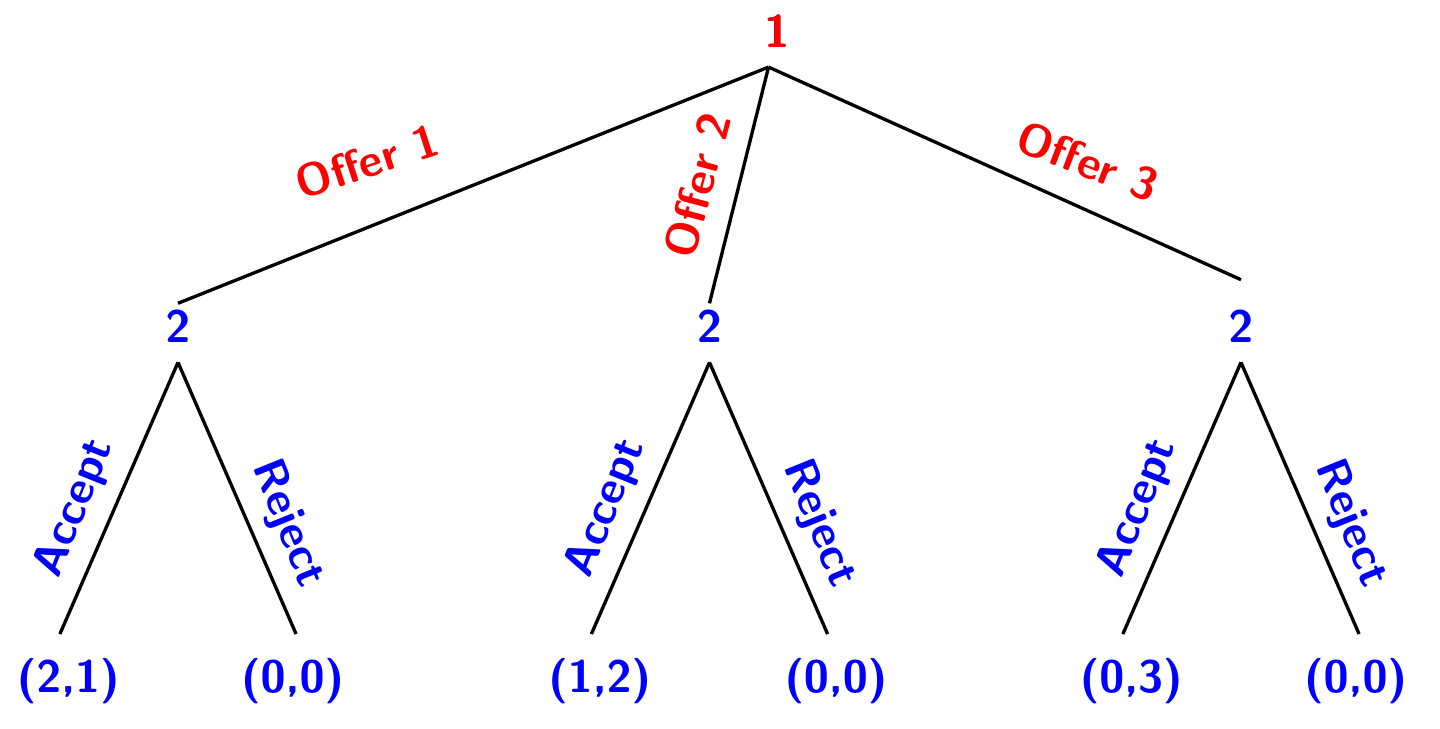
\includegraphics[
width=0.95\linewidth
]{../images/week03_01.png}

\end{center}



%=========================================================
\section{Pure Strategies and Normal Form}


\begin{definition}

\textbf{PURE STRATEGY (SEQUENTIAL GAME)}

A pure strategy for Player $i$ in a sequential game of perfect information is a
\textbf{contingent plan} that specifies an action at \textbf{each decision node} of
Player $i$.

\end{definition}


\begin{example}

Ultimatum game: a pure strategy for Player 1 could be simply ``Offer 1''. A pure strategy for
Player 2 could be ``Reject if the offer is 1 or 2, and accept if the offer is 3''.

\end{example}


\textbf{Normal-form representation of the Ultimatum game}

\begin{center}
\footnotesize
\setlength{\tabcolsep}{2pt}
\begin{tabular}{c|cccccccc}
$1 \backslash 2$ & RRR & RRA & RAA & AAA & ARR & RAR & AAR & ARA \\
\hline
Offer 1 & (0,0) & (0,0) & (0,0) & (2,1) & (2,1) & (0,0) & (2,1) & (2,1) \\
Offer 2 & (0,0) & (0,0) & (1,2) & (1,2) & (0,0) & (1,2) & (1,2) & (0,0) \\
Offer 3 & (0,0) & (0,3) & (0,3) & (0,3) & (0,0) & (0,0) & (0,0) & (0,3) \\
\end{tabular}
\end{center}


The eight choices for Player 2 are his eight possible pure strategies: e.g.\ `RRR' means
Reject if offered 1, 2 or 3; `RAR' means Reject if offered 1, Accept if offered 2, Reject if
offered 3.



\end{multicols}


\end{document}
